%% =====================================================================
%% MIRAGE: Optimal, Road-Graph-Native Location Obfuscation at City Scale,
%% and a Threat-Model-Aware Privacy Metric for IoT Smart Cities.
%% IEEE Computer Society journal format. Self-contained; figures in ./figures/.
%% Compile: tectonic paper.tex
%% =====================================================================
\documentclass[10pt,journal,compsoc]{IEEEtran}
\usepackage{amsmath,amssymb,amsfonts}
\usepackage{graphicx}
\usepackage{textcomp}
\usepackage{booktabs}
\usepackage{multirow}
\usepackage{url}
\usepackage{cite}
\usepackage{algorithmic}
\usepackage{algorithm}
\usepackage{array}
\usepackage{xcolor}
\usepackage{mathptmx}
\usepackage[hidelinks]{hyperref}
\graphicspath{{figures/}}
\hyphenation{op-tical net-works semi-conduc-tor IoT}
\begin{document}

\title{MIRAGE: Optimal, Road-Graph-Native Location Obfuscation at City Scale for
IoT Smart Cities}

\author{Pushkal~Gupta,
        Praagya~Garg,
        M.~Nagasai~Dattu,
        and~S.~Ebenezer~Juliet%
\IEEEcompsocitemizethanks{
\IEEEcompsocthanksitem The authors are with the School of Computer Science and
Engineering, Vellore Institute of Technology, Vellore 632014, India.\protect\\
E-mail: pushkalgupta2005@gmail.com; ebenezer.juliet@vit.ac.in.
\IEEEcompsocthanksitem Corresponding author: Pushkal Gupta.}%
\thanks{Manuscript prepared July 2026.}}

\markboth{Preprint}%
{Gupta \MakeLowercase{\textit{et al.}}: Optimal Road-Graph-Native Location Obfuscation for IoT Smart Cities}

\IEEEtitleabstractindextext{%
\begin{abstract}
IoT smart cities depend on continuous location reporting, and a large family of
obfuscation mechanisms---$k$-anonymity, differential privacy (DP), graph
constraints, temporal cloaking---has been proposed to protect it. Two questions
remain unanswered in a deployable, quantitative way. First, \emph{how much
privacy does each mechanism actually provide}, on a common, comparable scale and
against the threats it faces? Second, \emph{how far are these heuristics from the
best achievable privacy} on a real road network? We answer both. (1)~We adopt an
adversary-grounded privacy metric---the expected error of an optimal Bayesian
adversary, in metres---and instantiate it under two threat models, a snapshot
adversary and a Viterbi trajectory adversary with a Markov mobility prior,
showing that a single privacy scale is inadequate because the two adversaries
rank mechanisms differently. (2)~We introduce \textbf{MIRAGE}, the first
\emph{road-graph-native} optimal obfuscation mechanism that scales to a real
city. MIRAGE computes, per location, the release distribution that provably
maximises the Bayesian adversary's error subject to a utility budget, with the
distortion and adversary error measured as graph shortest-path distance; it is
made tractable by solving one small linear program per \emph{density-adaptive
local region}, turning an intractable $|V|^2$ program into $|V|$ tiny ones. On
real OpenStreetMap networks of two cities under three mobility datasets (Beijing:
GeoLife, T-Drive; Porto) we measure the \emph{price of heuristics}: at matched
utility, DP and $k$-anonymity leave $5\text{--}22\%$ of the achievable privacy on
the table in the operationally relevant regime, while MIRAGE is Pareto-optimal
(privacy$\,\approx\,$utility) up to the network's intrinsic uncertainty ceiling.
We further show rankings hold from a grid abstraction to the real network and that
service availability is dataset-density-driven rather than mechanism-intrinsic.
The complete framework---mechanisms, adversaries, datasets, and analysis---is
released for reproducibility.
\end{abstract}
\begin{IEEEkeywords}
Location privacy, optimal obfuscation, Bayesian adversary, differential privacy,
$k$-anonymity, road networks, trajectory privacy, Internet of Things.
\end{IEEEkeywords}}
\maketitle
\IEEEdisplaynontitleabstractindextext
\IEEEpeerreviewmaketitle

% =====================================================================
\section{Introduction}
\label{sec:intro}
% =====================================================================
\IEEEPARstart{S}{mart} cities collect fine-grained locations from IoT devices for
analytics, traffic management, and emergency response, and simultaneously expose
homes, workplaces, and mobility patterns \cite{sweeney2002}. Two decades of
research have produced diverse obfuscation mechanisms: spatial $k$-anonymity
\cite{gruteser2003}, differential privacy and geo-indistinguishability
\cite{dwork2006,andres2013}, graph-constrained perturbation \cite{bordenabe2014},
density adaptation \cite{niu2014}, and temporal cloaking \cite{gruteser2003}. Yet
a practitioner choosing a mechanism for a real deployment faces two unanswered
questions.

\emph{Q1: How private is each mechanism, comparably and against the right
threat?} Mechanisms are scored on incompatible, family-specific scales
($k/k_{\max}$, a log-scaled $\varepsilon$, region areas) that have no common
operational meaning and are usually measured against a single snapshot attacker,
even for mechanisms designed to defeat trajectory tracking.

\emph{Q2: How far are deployed heuristics from the best achievable privacy?}
Classical theory shows that, for a given utility budget, there exists an
\emph{optimal} obfuscation mechanism---the solution of a linear program (LP)---
that maximises a Bayesian adversary's error \cite{shokri2012,shokri2015pets,
bordenabe2014}. But that theory has only ever been instantiated on the Euclidean
plane or small grids, is snapshot-focused, and does not scale ($|V|^2$
variables), so it has never been evaluated on a real road network, and the gap
between deployable heuristics and the optimum on real topology is unknown.

We answer both questions.

\noindent\textbf{Contributions.}
\begin{enumerate}
\item \textbf{An adversary-grounded, threat-model-aware privacy metric}
(Section~\ref{sec:adversary}). Privacy is the expected error of an optimal
Bayesian adversary (Shokri~\emph{et~al.}~\cite{shokri2011}), in metres, evaluated
under both a snapshot adversary and a Viterbi trajectory adversary with a Markov
mobility prior. We show the two adversaries induce \emph{different} rankings, so
a single privacy scale is invalid.
\item \textbf{MIRAGE, the first road-graph-native optimal obfuscation mechanism
that scales to a real city} (Section~\ref{sec:mirage}). MIRAGE solves the
optimal-mechanism LP with graph shortest-path distortion and on-graph support,
made tractable by \emph{density-adaptive local LPs}. DP and $k$-anonymity arise
as constrained/degenerate special cases; an optional geo-indistinguishability
constraint recovers a formal DP guarantee.
\item \textbf{The price of heuristics on real road networks}
(Section~\ref{sec:results}). Across three mobility datasets on real networks of
two cities we quantify, at matched utility, how much privacy DP and $k$-anonymity
sacrifice ($5\text{--}22\%$ in the practical regime), with $95\%$ bootstrap CIs
and an ablation of MIRAGE's knobs.
\item \textbf{A reproducible, real-network, multi-city evaluation and open
framework} spanning a grid abstraction and real OSM graphs of Beijing and Porto,
three datasets (GeoLife, T-Drive, Porto taxi), and a radio-technology sensitivity
analysis of the energy model.\footnote{\url{https://github.com/Pushkal-Gupta/Graph-based-Location-Privacy-IoT}}
\end{enumerate}

Honest positioning: we do not invent optimal obfuscation---that is due to
Shokri~\emph{et~al.}~\cite{shokri2012,shokri2015pets} and Bordenabe~\emph{et~al.}
\cite{bordenabe2014}. Our contribution is to make it \emph{graph-native},
\emph{city-scale}, and \emph{measured} on real road networks, and to place it in
a unified two-threat evaluation.

% =====================================================================
\section{Related Work}
\label{sec:related}
% =====================================================================
\textbf{Heuristic mechanisms.} Spatial cloaking and $k$-anonymity
\cite{sweeney2002,gruteser2003,mokbel2006,duckham2005}, geo-indistinguishability
and the planar Laplace mechanism \cite{andres2013,chatzikokolakis2013}, graph
projection \cite{bordenabe2014}, density-aware $k$
\cite{niu2014}, and temporal cloaking \cite{gruteser2003} are all heuristics:
they fix a rule and accept whatever privacy it yields.

\textbf{Optimal mechanisms.} Shokri~\emph{et~al.}~\cite{shokri2012} showed the
utility-optimal mechanism against a Bayesian localization adversary is an LP;
\cite{shokri2015pets} casts it as a Stackelberg game; Bordenabe~\emph{et~al.}
\cite{bordenabe2014} add geo-indistinguishability as linear constraints. All are
on the Euclidean plane / regular grids, are snapshot-focused, and are explicitly
scalability-limited (the LP has $|V|^2$ variables); none is evaluated on a real
road network. MIRAGE closes exactly this gap.

\textbf{Trajectory correlation.} Xiao and Xiong \cite{xiao2015} showed per-report
DP degrades under Markov temporal correlation; subsequent work handles
trajectories via DP composition, dummies, or synthesis \cite{du2023,hu2024,
buchholz2024}. We use a Viterbi trajectory adversary to \emph{measure} this
degradation across mechanisms on a common scale.

\textbf{Quantifying privacy.} Shokri~\emph{et~al.}~\cite{shokri2011} define
location privacy as the expected error of an optimal adversary---the metric we
adopt for a comparable, in-metres evaluation.

% =====================================================================
\section{System Model and Threat Models}
\label{sec:sysmodel}
% =====================================================================
\textbf{Graph.} The environment is an undirected weighted graph $G=(V,E)$ with
edge weights the road distance and $d_G$ the shortest-path metric. We use two
graphs over central Beijing: a controlled $30\times30$ grid (900 nodes) that
removes topological confounds, and the \emph{real} OpenStreetMap drive network
for the same region, consolidated to $3{,}154$ nodes / $5{,}111$ edges with
irregular degree (mean $3.24$, max $23$), $16\%$ dead-ends, and hierarchy---
absent from the grid.

\textbf{Data.} Three real mobility datasets across two cities. In Beijing:
GeoLife \cite{zheng2009,zheng2008} ($182$ users, multi-modal GPS; $\sim$11.4\,M
points map-matched to the real graph) and T-Drive ($\sim$10k taxis; $\sim$4\,M
points), a much denser regime. In Porto, Portugal: the ECML/PKDD taxi dataset
($1.71$\,M trips, $\sim$81\,M points map-matched to a real Porto OSM graph of
$3{,}455$ nodes). Using multiple datasets of very different density, and a
\emph{second city}, separates mechanism properties from single-dataset or
single-city quirks.

\textbf{Two adversaries.} Both know the mechanism and public background
knowledge---a population prior $\pi(v)$ and a first-order Markov mobility model
$P(v_{t+1}\mid v_t)$, estimated once from the data and shared, so no mechanism is
advantaged. A \emph{snapshot} adversary observes one release; a \emph{trajectory}
adversary observes a sequence and decodes it (Section~\ref{sec:adversary}).

% =====================================================================
\section{Adversary-Grounded Privacy Metric}
\label{sec:adversary}
% =====================================================================
Privacy is the expected error of an optimal adversary that inverts the mechanism
using public knowledge \cite{shokri2011}, measured in metres and thus comparable
across all families.

\textbf{Snapshot adversary.} Observing release $o$, it forms the posterior
$P(v\mid o)\propto P(o\mid v)\,\pi(v)$ and outputs the Bayes estimate
$\hat v=\arg\min_{v'}\sum_v P(v\mid o)\,d_G(v',v)$; privacy is
$\mathbb{E}[d_G(v_{\text{true}},\hat v)]$. The observation model $P(o\mid v)$
differs by mechanism, but the measured quantity is identical.

\textbf{Trajectory adversary.} Observing a sequence, it Viterbi-decodes the
hidden node sequence, combining the per-report emission with the Markov prior;
privacy is the mean tracking error and per-step re-identification rate. This is
the threat temporal mechanisms target and that per-report noise fails against
\cite{xiao2015}.

\textbf{A single scale is inadequate.} Fig.~\ref{fig:dual} plots the two errors
against each other on the grid: density-aware adaptation and temporal cloaking
\emph{swap} rank between the threats, so any single-scale privacy comparison
mis-ranks mechanisms defending different threats.

\begin{figure}[t]\centering
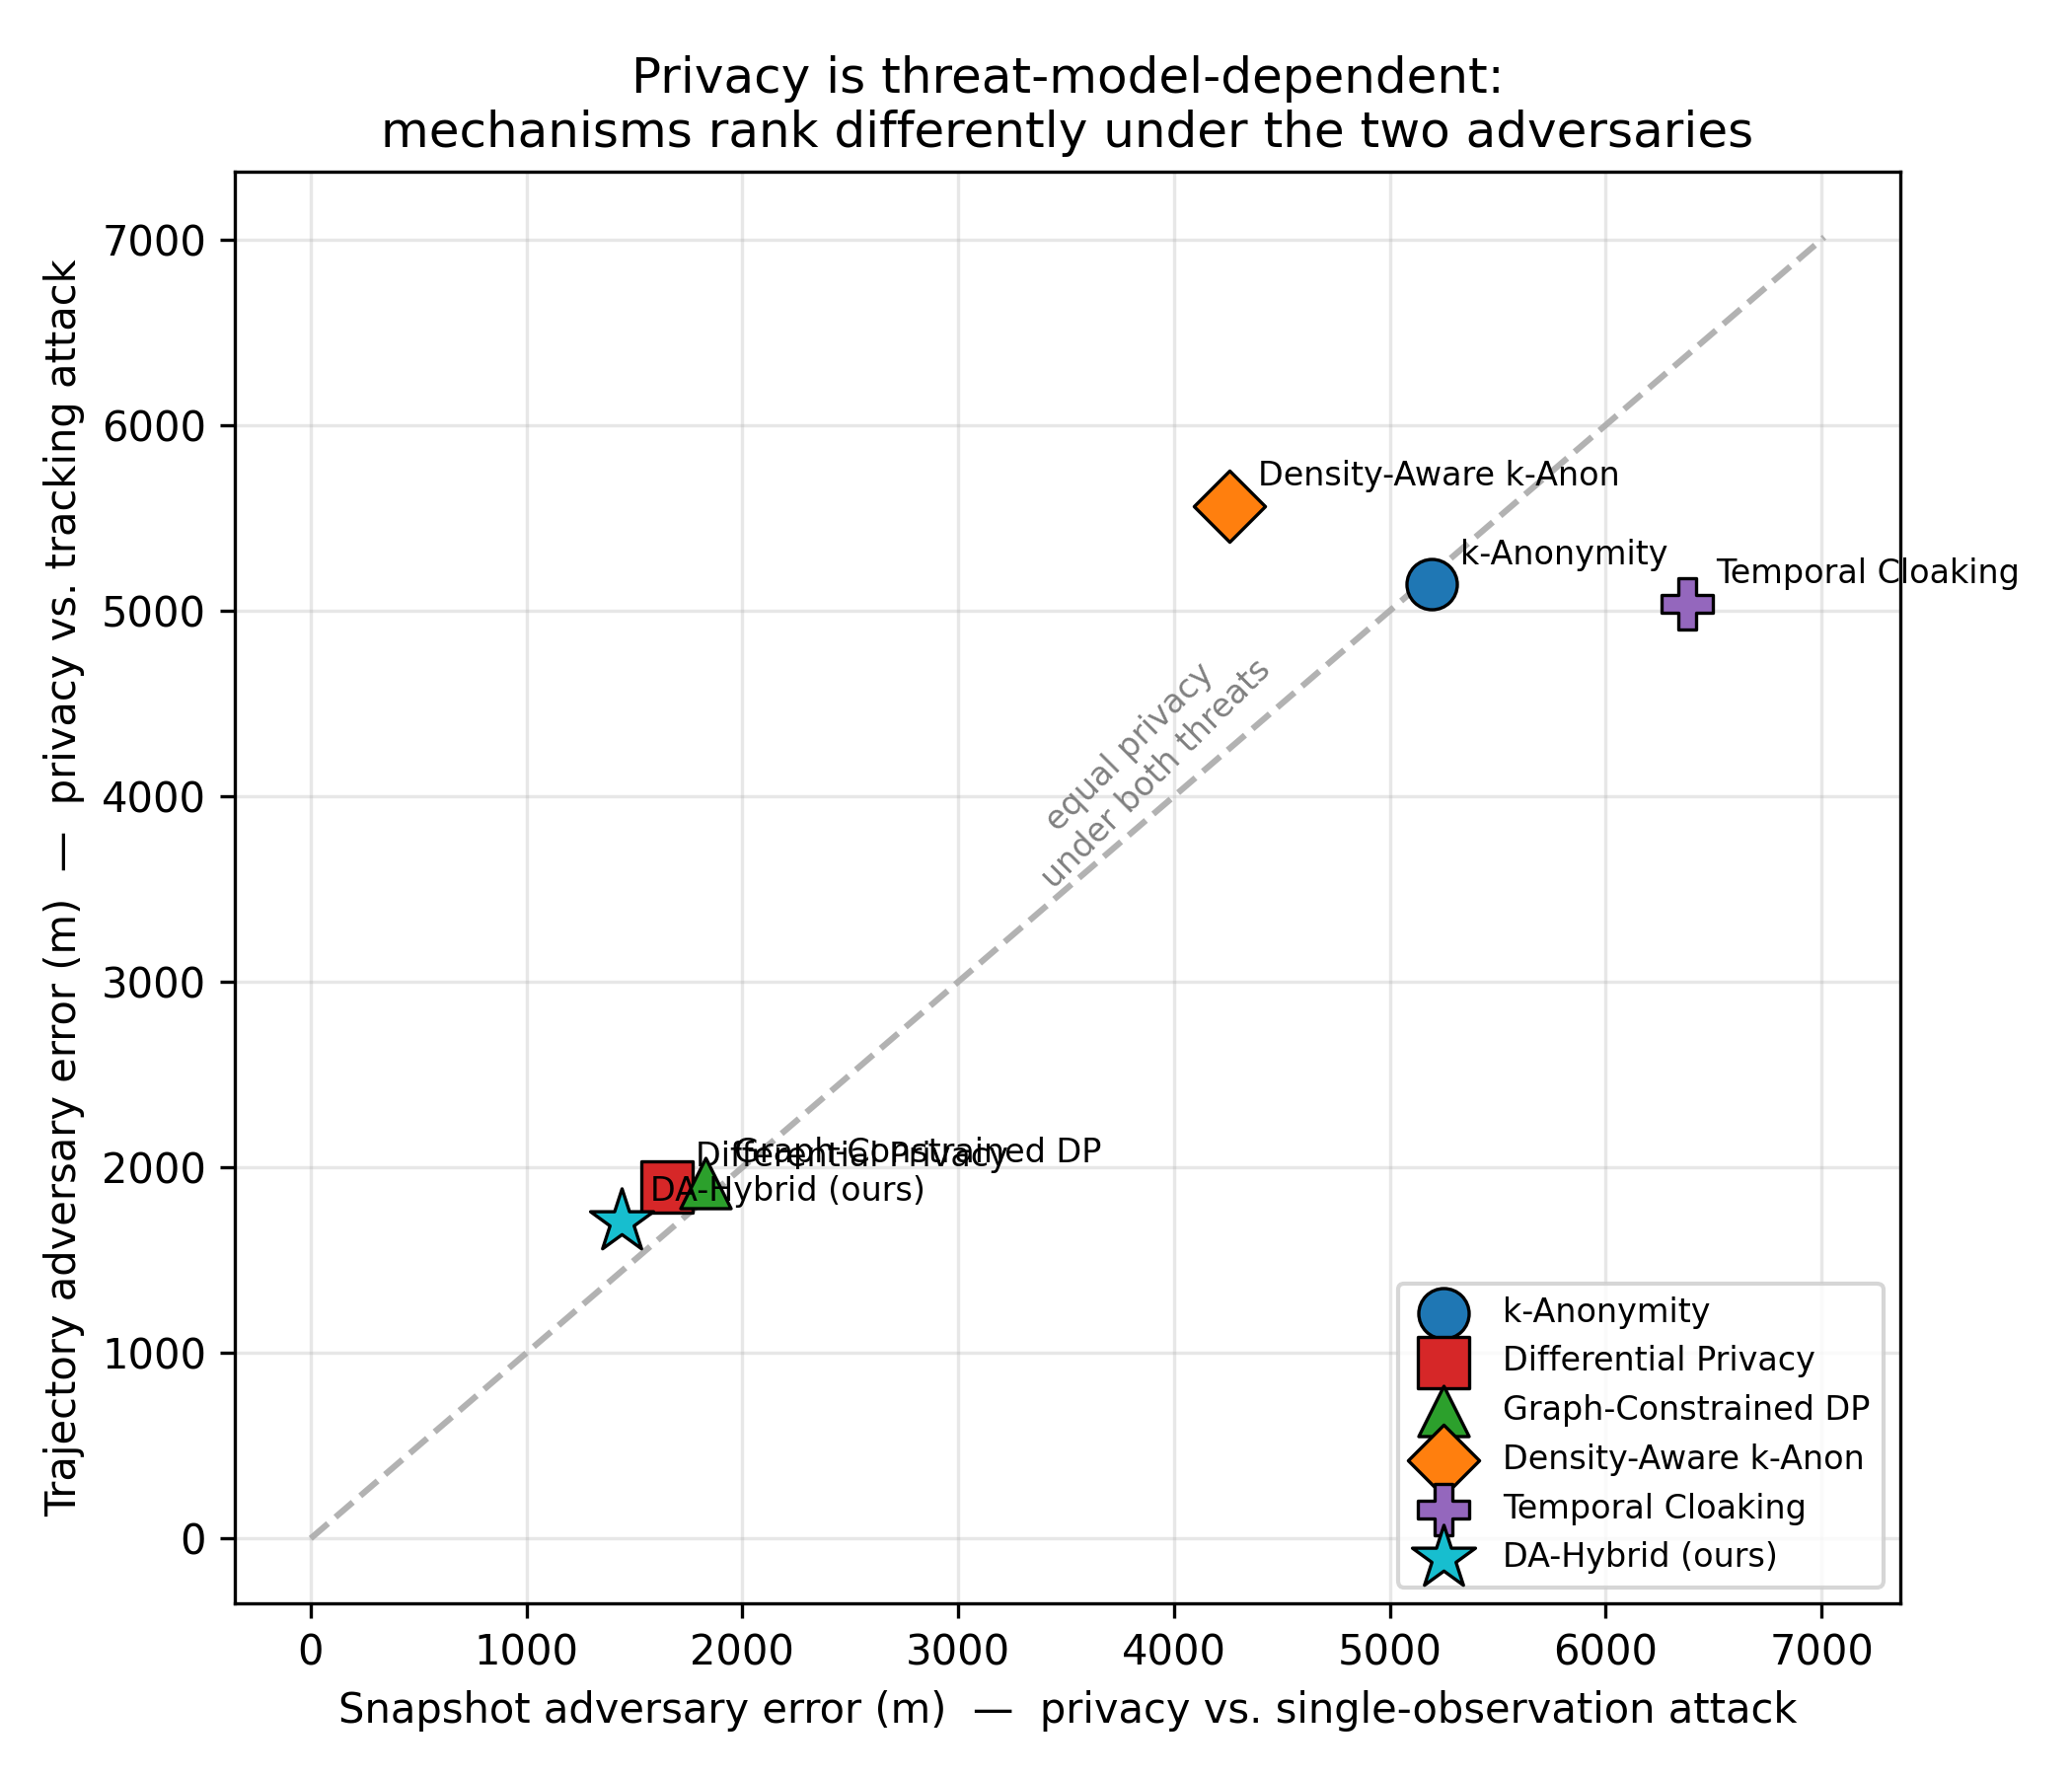
\includegraphics[width=0.95\columnwidth]{fig_dual_threat.png}
\caption{Privacy is threat-model dependent: mechanisms rank differently under the
snapshot ($x$) and trajectory ($y$) adversaries; points off the diagonal are
protected asymmetrically.}
\label{fig:dual}
\end{figure}

% =====================================================================
\section{MIRAGE: Optimal Graph-Native Obfuscation}
\label{sec:mirage}
% =====================================================================
\subsection{The Optimal Mechanism on a Graph}
For a prior $\pi$ and a utility (distortion) budget $D_{\max}$, the release
distribution $f(o\mid v)$ maximising the optimal Bayesian adversary's error, with
both distortion and adversary error measured in graph distance $d_G$, is the LP
\begin{align}
\max_{f,\,y}\ & \textstyle\sum_o y_o &&\text{(privacy, metres)}\label{eq:obj}\\
\text{s.t. }\ & y_o \le \textstyle\sum_v \pi(v)\,f(o\mid v)\,d_G(h,v)\ \ \forall o,h &&\text{(adversary)}\nonumber\\
& \textstyle\sum_v \pi(v)\sum_o f(o\mid v)\,d_G(v,o) \le D_{\max} &&\text{(utility)}\nonumber\\
& \textstyle\sum_o f(o\mid v)=1,\ f\ge 0. &&\nonumber
\end{align}
The auxiliary $y_o$ linearises the adversary's inner minimisation
(Shokri~\emph{et~al.}~\cite{shokri2012}); we instantiate it with $d_G$ and
on-graph output support, which is new. An optional geo-indistinguishability
constraint $f(o\mid v)\le e^{\varepsilon d_G(v,v')} f(o\mid v')$ adds a formal
$\varepsilon$-DP guarantee, recovering \cite{bordenabe2014} as a special case.

\subsection{Scaling to a City: Density-Adaptive Local LPs}
Program~\eqref{eq:obj} has $|V|^2$ variables---$\sim$$10^7$ for our graph---and is
intractable directly. MIRAGE partitions $V$ into \emph{density-adaptive local
regions}: starting from the highest-prior unassigned node, each region takes its
$C$ nearest still-unassigned nodes (dense areas are seeded first and covered by
tighter regions). We solve one LP of size $C$ per region and assign every member
its optimal row. This turns an $|V|^2$ program into $\lceil |V|/C\rceil$ programs
of $O(C^3)$ each---seconds to precompute offline, then $O(1)$ sampling at release
time. Releasing across regions is never optimal under a distortion budget (it
costs too much), so the partition is a principled, near-lossless approximation.

\begin{algorithm}[t]
\caption{MIRAGE precompute (per graph, offline)}
\label{alg:mirage}
\begin{algorithmic}[1]
\REQUIRE graph $G$, prior $\pi$, budget $D_{\max}$, region size $C$
\STATE partition $V$ into local regions (greedy, densest-first)
\FOR{each region $R$}
  \STATE $d_R \leftarrow$ graph distances on $R$; $\pi_R\leftarrow$ prior on $R$ (renorm.)
  \STATE $f_R \leftarrow$ solve LP~\eqref{eq:obj}$(d_R,\pi_R,D_{\max})$
  \STATE store $f_R(\cdot\mid v)$ for each $v\in R$
\ENDFOR
\end{algorithmic}
\end{algorithm}

DP, $k$-anonymity, and our earlier density-adaptive hybrid (DA-Hybrid) are
heuristic baselines; MIRAGE dominates them by construction and, we show, in
measurement.

% =====================================================================
\section{Experimental Setup}
\label{sec:setup}
% =====================================================================
All mechanisms share the graph, data, prior, and distance layer. We evaluate two
ways. (i)~The \emph{frontier}: for each mechanism we compute privacy (optimal-
adversary error) and utility (expected distortion) \emph{analytically} on the
same regions, sweeping the mechanism's knob ($D_{\max}$ for MIRAGE, $\varepsilon$
for DP, $k$ for $k$-anonymity), with $95\%$ weighted-bootstrap CIs over regions.
(ii)~A \emph{deployment comparison}: all seven mechanisms at representative
operating points under the sampled snapshot and trajectory adversaries, reporting
availability and spatial error. The energy model is swept across radio
technologies (Section~\ref{sec:energy}). MIRAGE uses $C{=}28$ unless noted.

% =====================================================================
\section{Results}
\label{sec:results}
% =====================================================================
\subsection{The Price of Heuristics}
\label{sec:price}
Fig.~\ref{fig:frontier} shows the privacy--utility frontier on the real GeoLife
graph. MIRAGE hugs the ideal (privacy$\,=\,$utility) at low distortion and
dominates DP and $k$-anonymity throughout the practical regime; all mechanisms
converge at high distortion to the network's intrinsic prior-uncertainty ceiling
($\sim$720\,m, the maximum error any mechanism can induce). Table~\ref{tab:price}
quantifies the gap: at matched utility, MIRAGE delivers $+13$ to $+22\%$ more
privacy than the best heuristic in the $150\text{--}500$\,m regime on GeoLife,
i.e., DP and $k$-anonymity waste that fraction of their distortion. The gap
closes only past $\sim$1100\,m, where all saturate at the ceiling.

\textbf{Cross-city generalisation.} The same result holds on all three datasets
and both cities (Fig.~\ref{fig:frontier_porto}): MIRAGE's gain over the best
heuristic in the practical regime is $+13$--$22\%$ on GeoLife, $+9$--$17\%$ on
T-Drive, and $+5$--$12\%$ on Porto. The magnitude tracks each city's mobility
structure---smaller where mobility is more predictable and heuristics are already
closer to optimal---but MIRAGE is Pareto-optimal and dominant in every setting.

\begin{figure}[t]\centering

\includegraphics[width=0.98\columnwidth]{fig_frontier_porto_real.png}
\caption{Cross-city check: privacy--utility frontier on the real Porto (Portugal)
network under the ECML/PKDD taxi dataset. MIRAGE dominates the heuristics here
too; the price of heuristics is $+5$--$12\%$ in the practical regime.}
\label{fig:frontier_porto}
\end{figure}

\begin{figure}[t]\centering
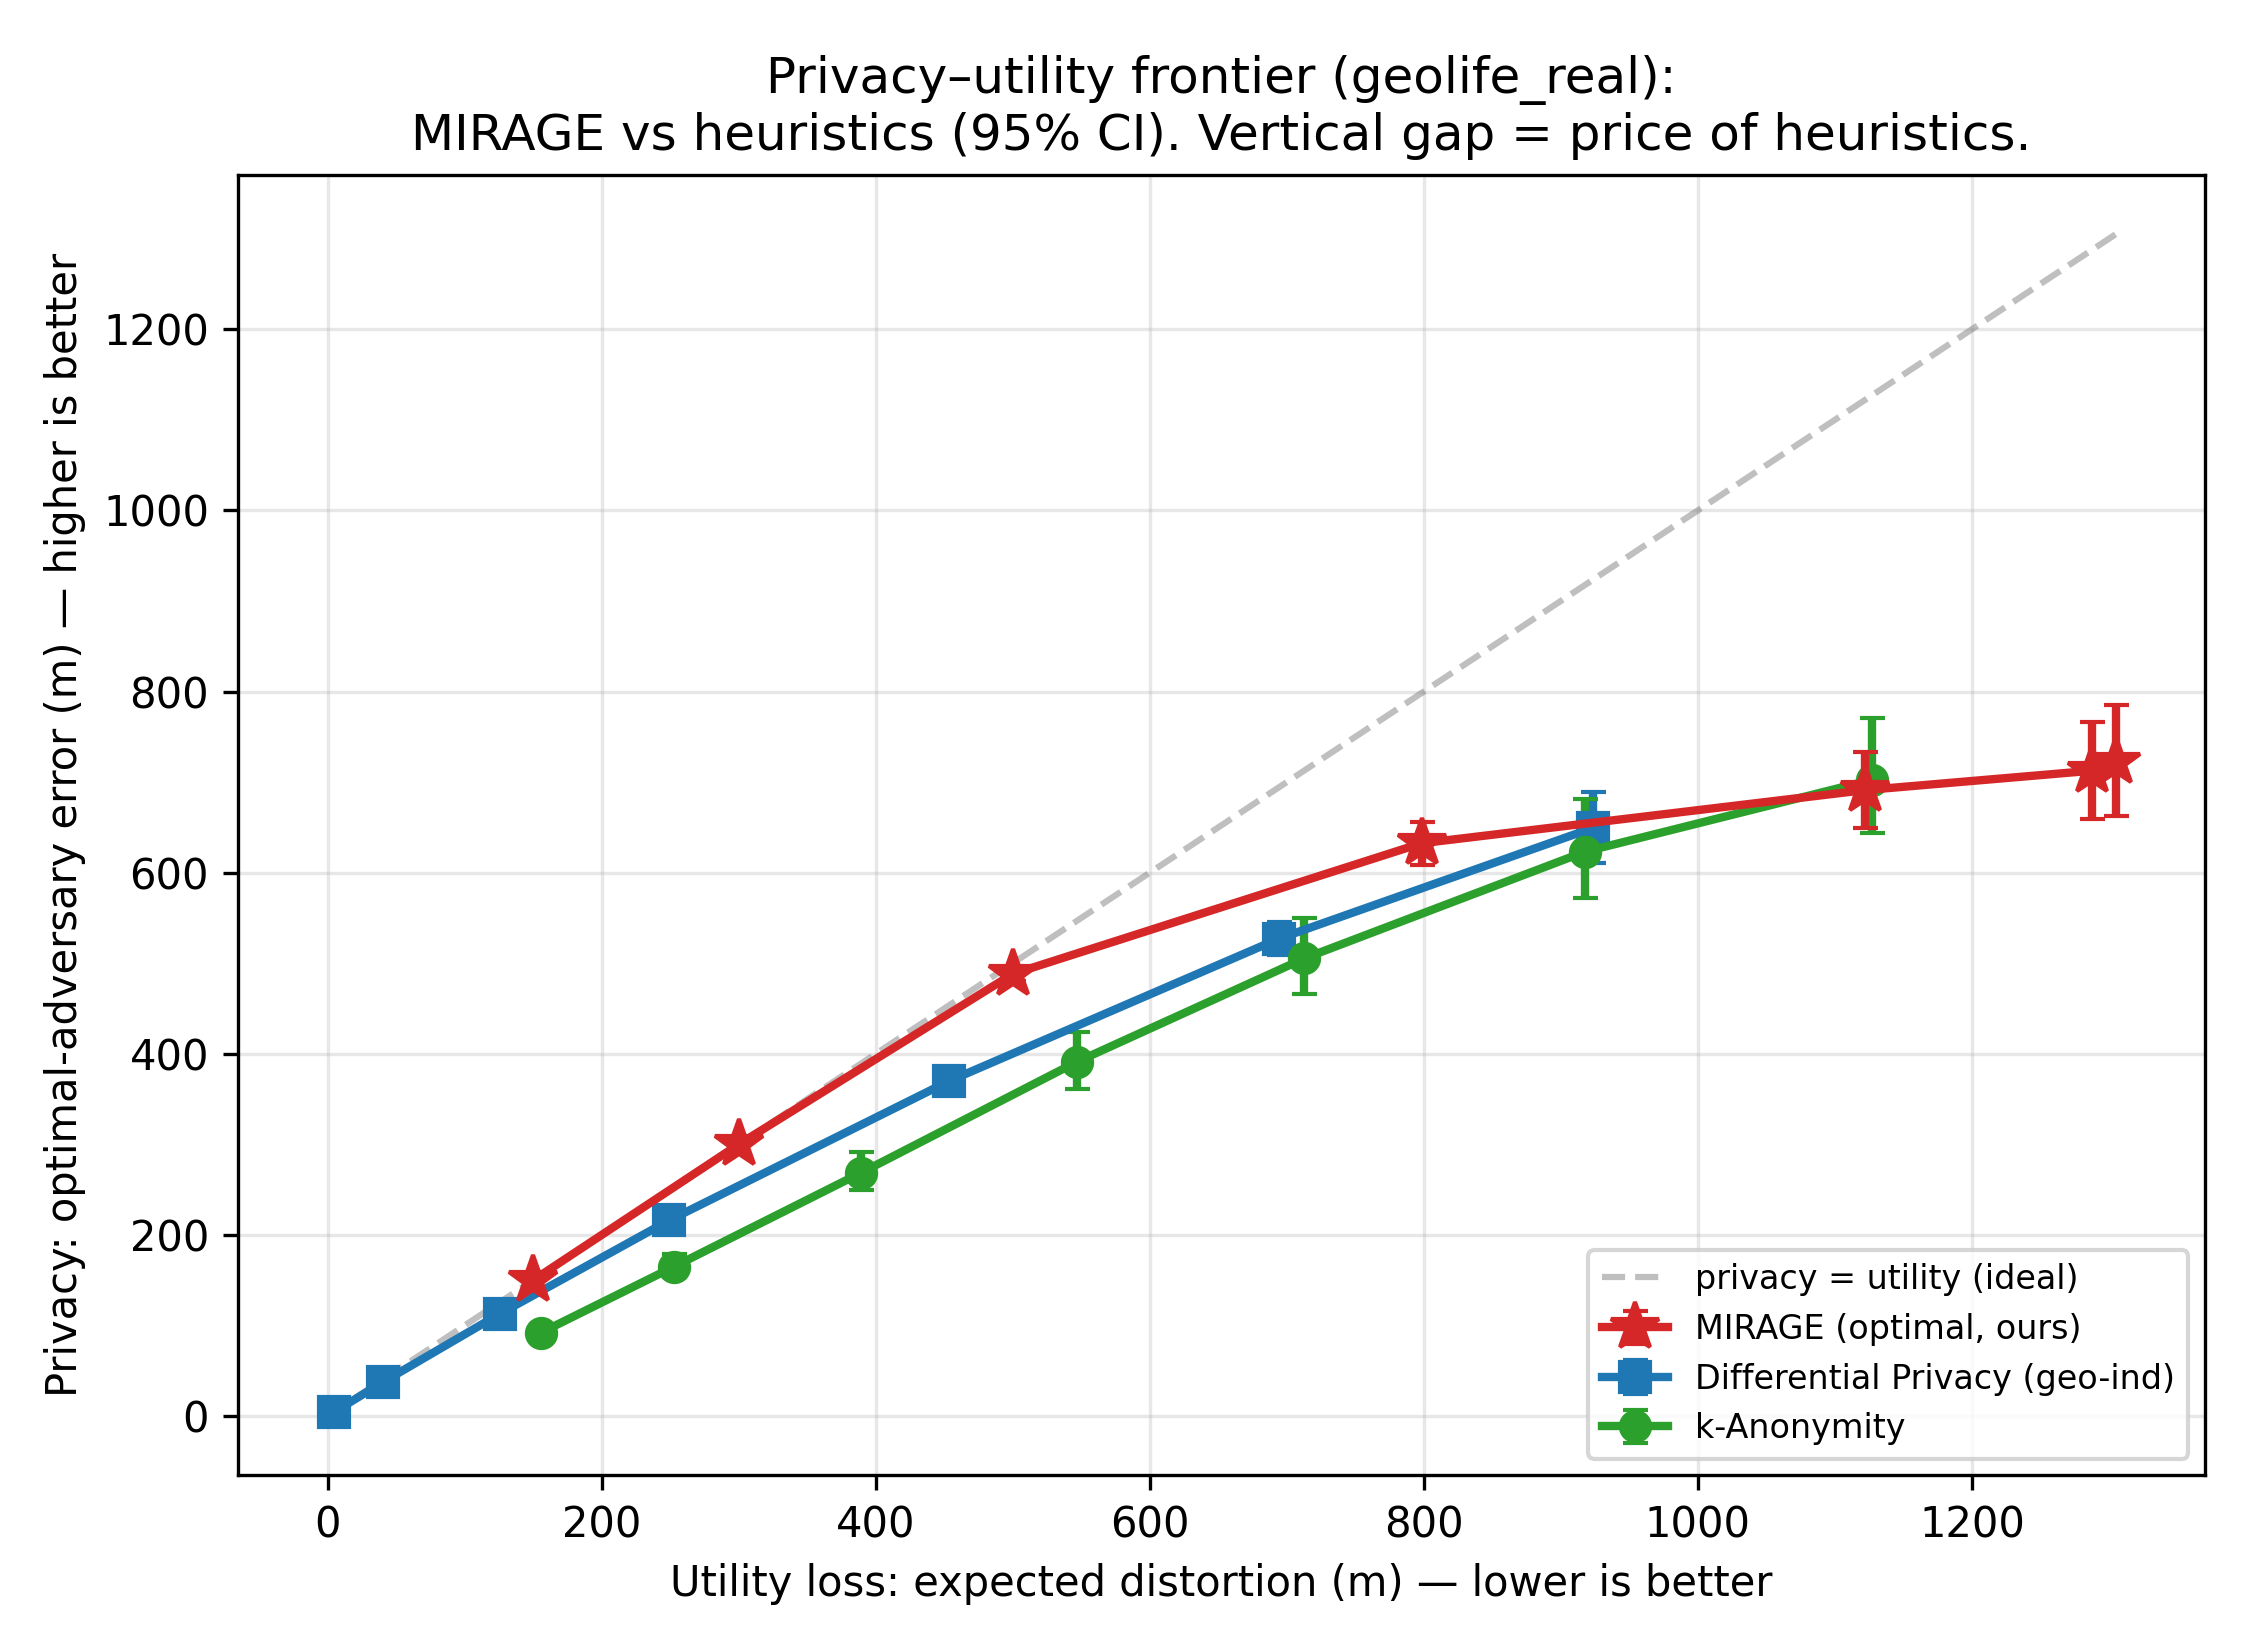
\includegraphics[width=0.98\columnwidth]{fig_frontier_geolife_real.png}
\caption{Privacy--utility frontier (GeoLife, real graph, $95\%$ CI). MIRAGE
(optimal) dominates the heuristics; the vertical gap to MIRAGE is the price of
heuristics. All converge at the intrinsic uncertainty ceiling.}
\label{fig:frontier}
\end{figure}

\begin{table}[t]\centering
\caption{Price of heuristics (GeoLife, real graph): privacy (optimal-adversary
error, m) at matched utility loss.}
\label{tab:price}
\begin{tabular}{rrrrr}
\toprule
Utility (m) & MIRAGE & DP & $k$-anon & MIRAGE gain \\
\midrule
150 & 150 & 133 & 92 & $+13\%$ \\
300 & 300 & 254 & 201 & $+18\%$ \\
500 & 488 & 400 & 355 & $+22\%$ \\
800 & 632 & 583 & 555 & $+9\%$ \\
$\ge$1100 & 700+ & 649 & 700+ & $\sim0\%$ (saturated) \\
\bottomrule
\end{tabular}
\end{table}

\subsection{Ablation: What Makes MIRAGE Work}
Table~\ref{tab:ablation} ablates the two knobs. Region size $C$ trades privacy
for LP time: privacy rises with $C$ (at $D_{\max}{=}800$: $421$\,m at $C{=}12$,
$632$\,m at $C{=}28$, $715$\,m at $C{=}40$) while solve time grows as $O(C^3)$
($1.3$\,s to $21$\,s over all regions); $C{=}28$ is the knee. The optional
geo-indistinguishability constraint costs some optimality ($632\!\to\!456$\,m at
$\varepsilon/\text{m}{=}0.01$) in exchange for a formal DP guarantee---MIRAGE
subsumes DP as its constrained case.

\begin{table}[t]\centering
\caption{MIRAGE ablation (GeoLife, real graph).}
\label{tab:ablation}
\begin{tabular}{lrrrr}
\toprule
Region size $C$ & 12 & 20 & 28 & 40 \\
\midrule
Privacy @ $D_{\max}{=}800$ (m) & 421 & 551 & 632 & 715 \\
LP time, all regions (s) & 1.3 & 3.1 & 7.0 & 20.8 \\
\bottomrule
\end{tabular}
\end{table}

\subsection{Deployment Comparison (All Mechanisms)}
Table~\ref{tab:main} compares all seven mechanisms on the real GeoLife graph
under the sampled snapshot and trajectory adversaries. MIRAGE serves every user
(100\% availability), is on-graph, and provides strong balanced privacy; the two
adversaries again reorder the heuristics. Two robustness findings emerge from
repeating on T-Drive: rankings hold under the adversary metric, and
\emph{availability is dataset-density-driven}---on dense T-Drive every mechanism
reaches 100\% availability, whereas on sparse GeoLife $k$-anonymity (33\%) and
density-aware (61\%) suffer denial of service (Fig.~\ref{fig:cross}).

\begin{table}[t]\centering
\caption{Deployment comparison (GeoLife, real graph, 10\,min). Privacy = Bayesian-
adversary error (m, higher = more private).}
\label{tab:main}
\begin{tabular}{lrrrr}
\toprule
Mechanism & Snap.\ AE & Traj.\ AE & Avail. & Loc.\ Err \\
\midrule
$k$-Anonymity & 1694 & 3459 & 33\% & 4493 \\
Differential Privacy & 730 & 947 & 100\% & 466 \\
Graph-Constr.\ DP & 1339 & 732 & 100\% & 1400 \\
Density-Aware & 1437 & 3459 & 61\% & 2379 \\
DA-Hybrid (heuristic) & 311 & 1885 & 100\% & 563 \\
Temporal Cloaking & 2577 & 4636 & 100\% & 3215 \\
\textbf{MIRAGE (ours)} & 846 & 855 & \textbf{100\%} & 1090 \\
\bottomrule
\end{tabular}
\end{table}

\begin{figure}[t]\centering

\includegraphics[width=\columnwidth]{fig_cross_topology.png}
\caption{Availability and error across the grid, the real graph (GeoLife), and
the real graph under T-Drive. Availability rises to 100\% for all mechanisms on
the dense dataset---it is density-driven, not mechanism-intrinsic.}
\label{fig:cross}
\end{figure}

\subsection{Energy-Model Sensitivity}
\label{sec:energy}
The claim that radio transmission dominates per-report energy holds only for
LPWAN/cellular radios (LoRa/NB-IoT/LTE-M, $99\%$ radio share) but not for BLE,
where computation is $6\text{--}50\%$ of energy for BFS-based mechanisms
(Fig.~\ref{fig:energy}). MIRAGE's release-time cost is a single categorical draw
($O(1)$), so it is as radio-dominated as DP.

\begin{figure}[t]\centering
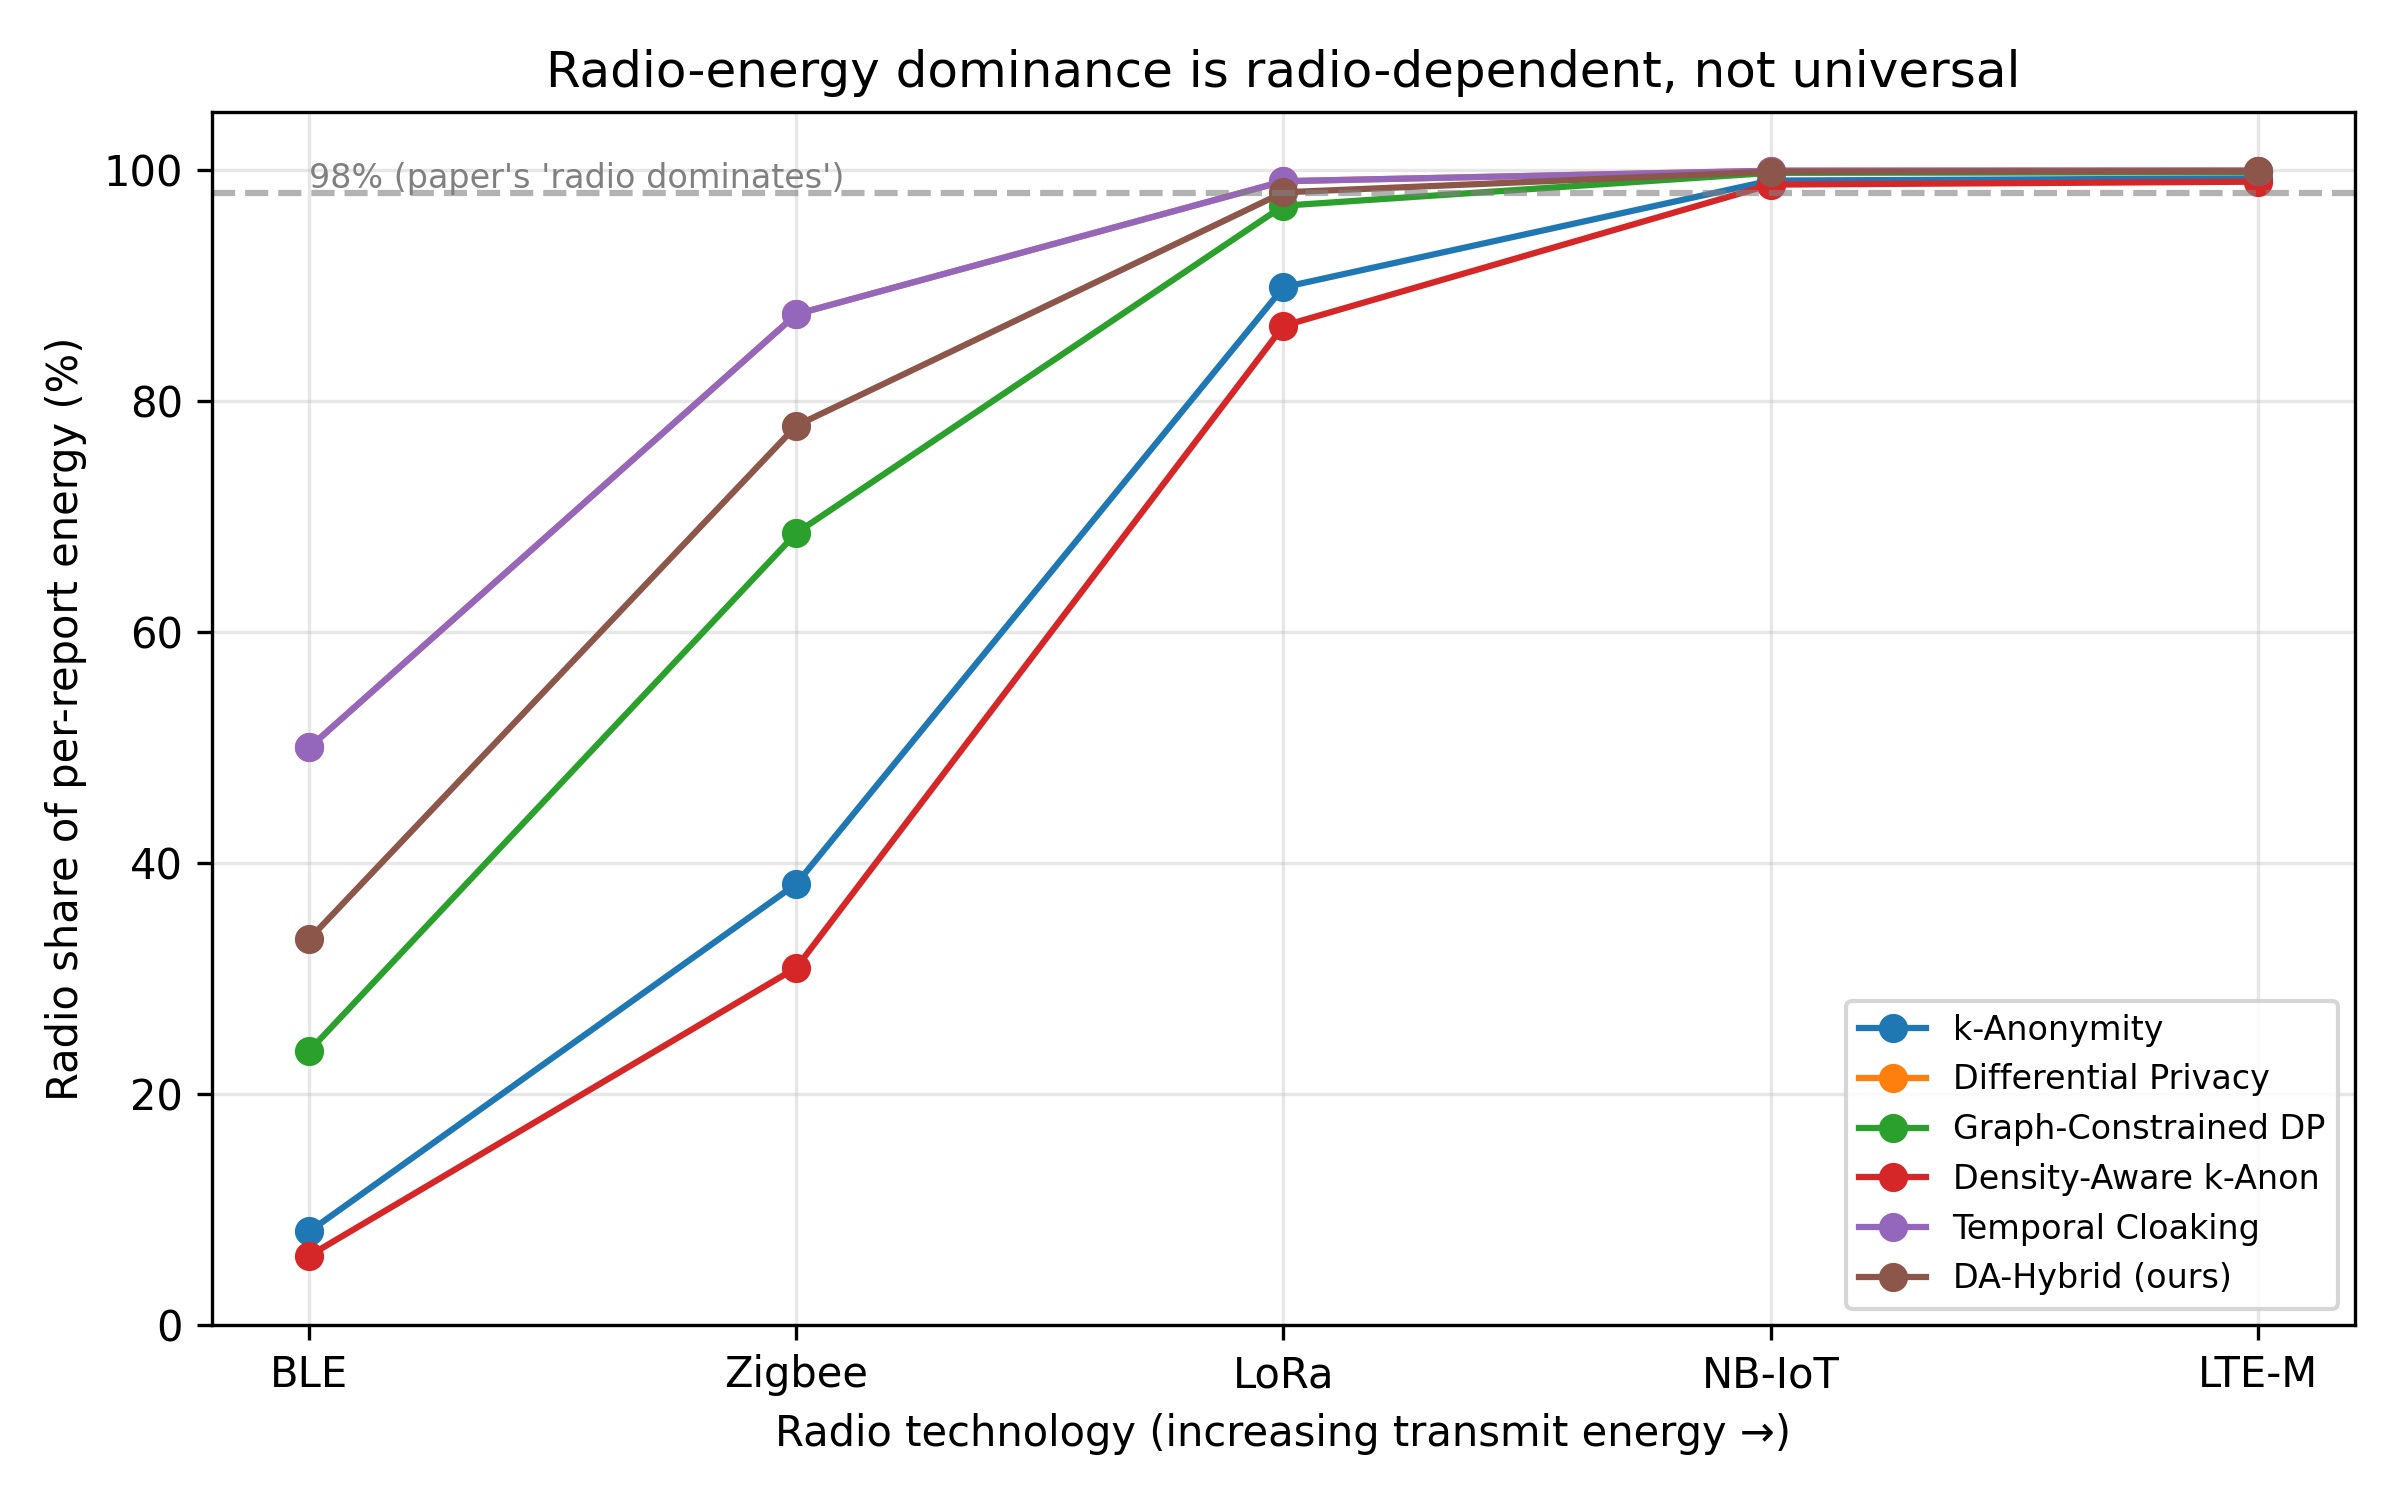
\includegraphics[width=0.95\columnwidth]{fig_energy_sensitivity.png}
\caption{Radio share of per-report energy vs radio technology. Radio dominance is
radio-dependent, not universal.}
\label{fig:energy}
\end{figure}

% =====================================================================
\section{Discussion}
\label{sec:discussion}
% =====================================================================
\textbf{Guidance.} MIRAGE gives, for a chosen utility budget on the operator's
own road network and mobility statistics, the release policy that provably
maximises attacker error---up to $+22\%$ more privacy than tuned heuristics at
equal utility, with 100\% availability and on-graph outputs. Where a formal DP
guarantee is required, its geo-indistinguishability-constrained variant applies
at a small, measured cost.

\textbf{Limitations (honest).} (i)~At high distortion the local-region cap ($C$)
bounds MIRAGE's reach, so heuristics catch up near the uncertainty ceiling;
hierarchical or overlapping regions would extend the advantage. (ii)~The
optimal-mechanism LP is per-snapshot; the trajectory adversary shows temporal
correlation still leaks, and a fully trajectory-optimal MIRAGE (optimising the
sequential adversary via a mobility-corrected objective) is promising future
work---the ``sequential estimation'' the name anticipates. (iii)~Absolute error
is graph-granularity dependent, so cross-topology conclusions rest on
adversary-privacy and availability. (iv)~The energy model is analytical, suited
to ranking; we report its radio sensitivity explicitly.

% =====================================================================
\section{Conclusion}
\label{sec:conclusion}
% =====================================================================
We measured location privacy on a common, adversary-grounded, threat-model-aware
scale and brought optimal obfuscation to a real road network at city scale with
MIRAGE. On real road networks of two cities across three datasets, deployed
heuristics leave $5\text{--}22\%$ of achievable privacy on the table in the
practical regime, while MIRAGE is Pareto-optimal with full availability and
on-graph outputs.
Rankings hold from grid to real topology, and availability is shown to be
dataset-density-driven. The framework is released for reproducible extension.

% =====================================================================
\begin{thebibliography}{99}
% =====================================================================
\bibitem{sweeney2002} L.~Sweeney, ``$k$-Anonymity: A model for protecting
privacy,'' \emph{Int. J. Uncertainty, Fuzziness Knowl.-Based Syst.}, vol.~10,
no.~5, pp.~557--570, 2002.
\bibitem{gruteser2003} M.~Gruteser and D.~Grunwald, ``Anonymous usage of
location-based services through spatial and temporal cloaking,'' in \emph{Proc.
MobiSys}, 2003, pp.~31--42.
\bibitem{dwork2006} C.~Dwork, ``Differential privacy,'' in \emph{Proc. ICALP},
LNCS 4052, 2006, pp.~1--12.
\bibitem{shokri2011} R.~Shokri, G.~Theodorakopoulos, J.-Y.~Le Boudec, and
J.-P.~Hubaux, ``Quantifying location privacy,'' in \emph{Proc. IEEE S\&P}, 2011,
pp.~247--262.
\bibitem{shokri2012} R.~Shokri, G.~Theodorakopoulos, C.~Troncoso, J.-P.~Hubaux,
and J.-Y.~Le Boudec, ``Protecting location privacy: Optimal strategy against
localization attacks,'' in \emph{Proc. ACM CCS}, 2012, pp.~617--627.
\bibitem{shokri2015pets} R.~Shokri, ``Privacy games: Optimal user-centric data
obfuscation,'' \emph{Proc. Privacy Enhancing Technologies}, vol.~2015, no.~2,
pp.~299--315, 2015.
\bibitem{bordenabe2014} N.~E.~Bordenabe, K.~Chatzikokolakis, and C.~Palamidessi,
``Optimal geo-indistinguishable mechanisms for location privacy,'' in \emph{Proc.
ACM CCS}, 2014, pp.~251--262.
\bibitem{andres2013} M.~E.~Andr\'{e}s, N.~E.~Bordenabe, K.~Chatzikokolakis, and
C.~Palamidessi, ``Geo-indistinguishability: Differential privacy for
location-based systems,'' in \emph{Proc. ACM CCS}, 2013, pp.~901--914.
\bibitem{chatzikokolakis2013} K.~Chatzikokolakis \emph{et~al.}, ``Broadening the
scope of differential privacy using metrics,'' in \emph{Proc. PETS}, 2013,
pp.~82--102.
\bibitem{mokbel2006} M.~F.~Mokbel, C.-Y.~Chow, and W.~G.~Aref, ``The new Casper:
Query processing for location services without compromising privacy,'' in
\emph{Proc. VLDB}, 2006, pp.~763--774.
\bibitem{duckham2005} M.~Duckham and L.~Kulik, ``A formal model of obfuscation
and negotiation for location privacy,'' in \emph{Pervasive Computing}, LNCS 3468,
2005, pp.~152--170.
\bibitem{niu2014} B.~Niu, Q.~Li, X.~Zhu, G.~Cao, and H.~Li, ``Achieving
$k$-anonymity in privacy-aware location-based services,'' in \emph{Proc. IEEE
INFOCOM}, 2014, pp.~754--762.
\bibitem{xiao2015} Y.~Xiao and L.~Xiong, ``Protecting locations with differential
privacy under temporal correlations,'' in \emph{Proc. ACM CCS}, 2015,
pp.~1298--1309.
\bibitem{du2023} Y.~Du \emph{et~al.}, ``LDPTrace: Locally differentially private
trajectory synthesis,'' \emph{Proc. VLDB Endow.}, vol.~16, no.~8, pp.~1897--1909,
2023.
\bibitem{hu2024} Y.~Hu \emph{et~al.}, ``Real-time trajectory synthesis with local
differential privacy,'' in \emph{Proc. IEEE ICDE}, 2024, pp.~1685--1698.
\bibitem{buchholz2024} E.~Buchholz \emph{et~al.}, ``SoK: Can trajectory
generation combine privacy and utility?,'' \emph{Proc. PETS}, vol.~2024, no.~3,
pp.~75--93, 2024.
\bibitem{zheng2009} Y.~Zheng, L.~Zhang, X.~Xie, and W.-Y.~Ma, ``Mining
interesting locations and travel sequences from GPS trajectories,'' in \emph{Proc.
WWW}, 2009, pp.~791--800.
\bibitem{zheng2008} Y.~Zheng, Q.~Li, Y.~Chen, X.~Xie, and W.-Y.~Ma,
``Understanding mobility based on GPS data,'' in \emph{Proc. UbiComp}, 2008,
pp.~312--321.
\end{thebibliography}
\end{document}
